\newpage
% \renewcommand{\labelenumi}{\latintext{enumi}}
\section{Задание 1}
 {\bf\large Условие} \\Построить эскиз графика данной функции, используя преобразования
графика соответствующей \\ элементарной функции. Указать область определения и область значений данной функции:
\begin{enumerate}
    \item $y =3\sin{\left(2+\frac{x}{2\pi}\right)}-5$
    \item $y =\sqrt{\left(\frac{|6-2x|+x}{10-|5x-15|}\right)^2}$
    \item $y =\log_4{\left(2+\sqrt{\frac{1}{x}}\right)}$
\end{enumerate}
{\bf\large Ход решения} 
\[
    y =3\sin{\left(2+\frac{x}{2\pi}\right)}-5 = 3\sin{\left(\frac{(x+4\pi)}{2\pi}\right)}-5
\]
Построим базовую функцию: $y = \sin{x}$: \\
\begin{center}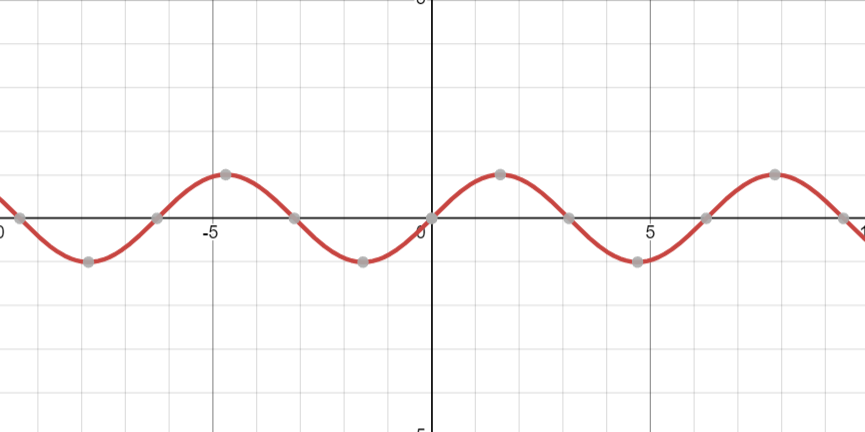
\includegraphics[width=0.7\linewidth]{1.png}\end{center}
Изменим циклическую частоту: $y = \sin{\left(\frac{x}{2\pi}\right)}$: \\
\begin{center}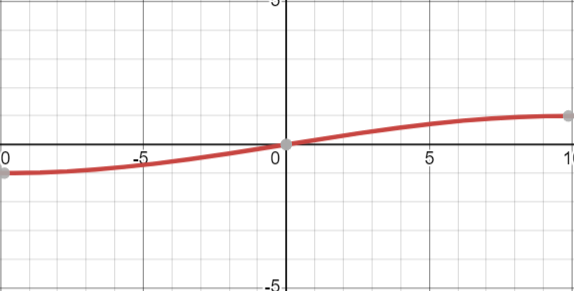
\includegraphics[width=0.7\linewidth]{2.png}\end{center}
Растянем график в 3 раза по OY: $y = 3\sin{\left(\frac{x}{2\pi}\right)}$:
\begin{center}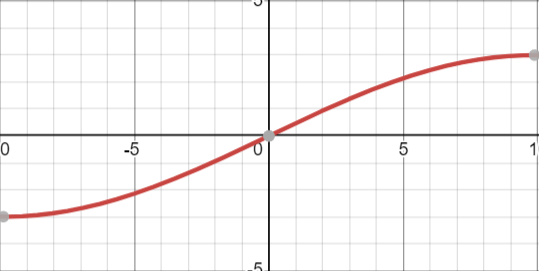
\includegraphics[width=0.7\linewidth]{3.png}\end{center}
Построим график относительно новых осей: 
$y' = y + 5$ и $x' = x + 4\pi$:
\begin{center}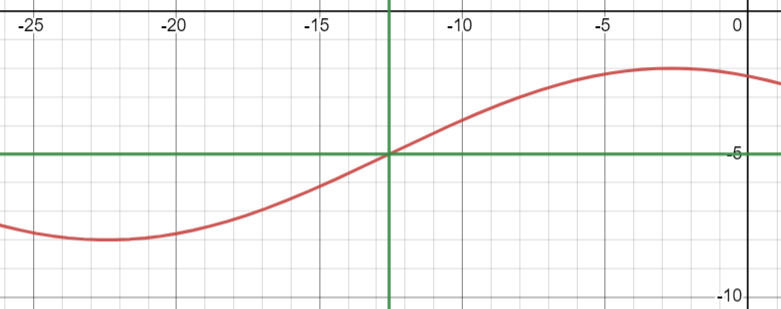
\includegraphics[width=0.7\linewidth]{4.png}\end{center}
В итоге, посредством элементарных преобразований мы получили график функции $y =3\sin{\left(2+\frac{x}{2\pi}\right)}-5$:
\begin{center}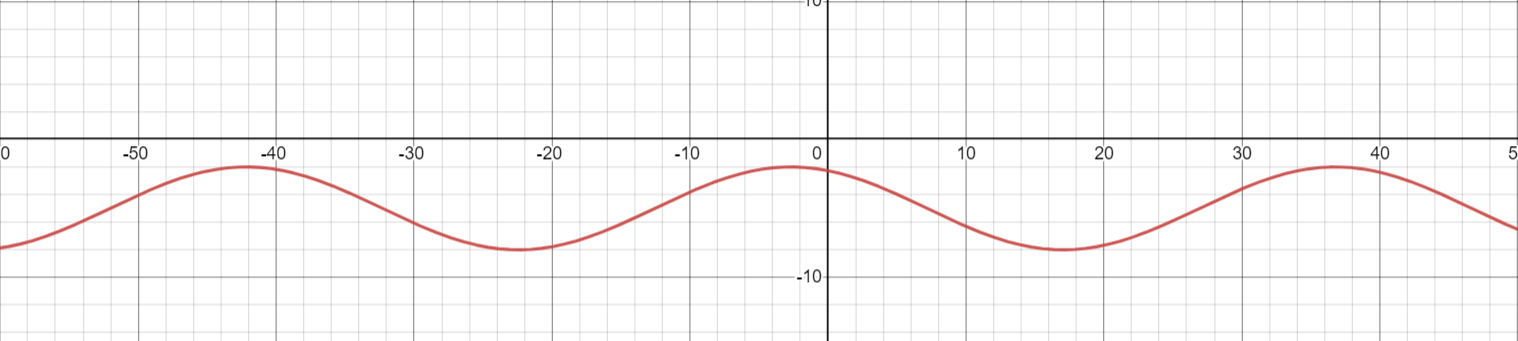
\includegraphics[width=0.7\linewidth]{5.png}\end{center}
\newpage



